% Content of Worksheet 04, shared by the problem sheet and the solution sheet.
% Solutions are wrapped in the `solution` environment and appear only when the
% driver defines \ipsshowsolutions.

\ipsmaketitle

This worksheet is ungraded practice, with the same shape and level as the final exam.
Plan up to 2 hours for a serious pass.
Work each problem through on paper before you open the solutions, and show your algebra:
the exam asks for the steps, not only the number.
Some parts state an intermediate result (``show that\,\ldots''); use it to check your work, and to continue if a step resists.
Carry at least four significant figures through the intermediate steps (the worked solutions print five) and round only at the end.
All parts are analytical; no computer is needed.

\begin{given}[Constants and data]
$G = 6.674 \times 10^{-11}\ \mathrm{m^3\,kg^{-1}\,s^{-2}}$

\vskip4pt
Mars: $M = 6.417 \times 10^{23}$ kg, $R = 3389.5$ km, $g = 3.71\ \mathrm{m\,s^{-2}}$

\vskip4pt
Moon: $R = 1737$ km, $g = 1.62\ \mathrm{m\,s^{-2}}$, simple-to-complex transition $D_t \approx 15$ km, core radius $200$--$380$ km

\vskip4pt
Mercury: $\bar\rho = 5427\ \mathrm{kg\,m^{-3}}$, core radius fraction $x = r_c/R = 0.83$, core mass fraction $0.74$

\vskip6pt
\begin{tabular}{@{}lccccc@{}}
\toprule
 & Uniform sphere & Moon & Mars & Mercury & Earth \\
\midrule
$C/MR^2$ & 0.400 & 0.393 & 0.364 & 0.346 & 0.331 \\
\bottomrule
\end{tabular}

\vskip4pt
{\footnotesize Interior data as in the Lecture 8 notes; crater scaling and chronology as in the Lecture 7 notes. Take $\rho = 3000\ \mathrm{kg\,m^{-3}}$ for rocky impactors and for the martian target surface.}
\end{given}


% ════════════════════════════════════════════════════════════
\problem{Impact energetics on Mars}

Impact craters are the default landform of the solar system,
and a single scaling law connects the size of a crater to the energy of the impactor that made it.

\parti A rocky asteroid of diameter $400$ m ($\rho = 3000\ \mathrm{kg\,m^{-3}}$) strikes Mars at $v = 12\ \mathrm{km\,s^{-1}}$.
Compute its mass and kinetic energy,
then the crater diameter from the gravity-regime scaling
\[
D \approx \left(\frac{E_k}{\rho_t\,g}\right)^{1/4},
\]
with $\rho_t$ the target density (show that $D \approx 5.05$ km).

\begin{solution}
The impactor radius is $200$ m, so
\[
m = \frac{4}{3}\pi r^3 \rho = \frac{4}{3}\pi\,(200)^3 \times 3000 = 1.0053 \times 10^{11}\ \mathrm{kg},
\]
and the kinetic energy is
\[
E_k = \tfrac{1}{2} m v^2 = 0.5 \times 1.0053 \times 10^{11} \times (1.2 \times 10^{4})^2 = 7.2382 \times 10^{18}\ \mathrm{J}.
\]
The scaling argument then gives
\[
\frac{E_k}{\rho_t\,g} = \frac{7.2382 \times 10^{18}}{3000 \times 3.71} = 6.5033 \times 10^{14}\ \mathrm{m^4},
\qquad
D = \left(6.5033 \times 10^{14}\right)^{1/4} = 5049.9\ \mathrm{m} \approx 5.05\ \mathrm{km},
\]
matching the checkpoint: a $400$ m body excavates a crater more than twelve times its own size.
\answer{$m = 1.0053 \times 10^{11}\ \mathrm{kg}$, $E_k = 7.2382 \times 10^{18}\ \mathrm{J}$, and $D = 5049.9\ \mathrm{m} \approx 5.05\ \mathrm{km}$. A $400$ m body excavates a crater more than twelve times its own size.}
\end{solution}

\parti Show from the scaling law that, at fixed impact speed and densities, the crater diameter grows with the impactor diameter $L$ as $D \propto L^{3/4}$.
Then invert the relation: what impactor diameter does a $50$ km martian crater require?
Comment on how strongly the fourth root compresses the mapping from impactor size to crater size.

\begin{solution}
At fixed $v$ and $\rho$, the impactor mass scales as $m \propto L^3$, so $E_k \propto L^3$, and the scaling law gives
\[
D \propto E_k^{1/4} \propto L^{3/4}.
\]
Inverting, $L_2 = L_1 (D_2/D_1)^{4/3}$. With $L_1 = 400$ m and $D_1 = 5.05$ km from part (a):
\[
L_2 = 400 \times \left(\frac{50}{5.05}\right)^{4/3} = 400 \times 21.260 = 8504\ \mathrm{m} \approx 8.5\ \mathrm{km}.
\]
The compression is strong in both directions: a crater ten times larger needs an impactor only about twenty times larger,
and equivalently a factor of $10^4$ in impact energy moves the crater diameter by only a factor of $10$.
This is why crater populations span such a wide range of sizes on every surface.
Read $L$ as an order of magnitude, not a measurement, as the Lecture 7 notes caution for Tycho: the scaling describes the transient cavity in the gravity regime, a $50$ km crater is complex and its final rim was widened by collapse, and the prefactor in the law is not fixed by dimensional analysis.
\answer{$D \propto L^{3/4}$, giving $L_2 = 8504\ \mathrm{m} \approx 8.5\ \mathrm{km}$ for a $50$ km crater. A factor of $10^4$ in impact energy moves the crater diameter by only a factor of $10$.}
\end{solution}

\parti The simple-to-complex transition diameter scales inversely with surface gravity,
\[
D_t \approx D_{t,\mathrm{Moon}}\,\frac{g_{\mathrm{Moon}}}{g}.
\]
Locate the transition on Mars, classify the crater from part (a) as simple or complex,
and explain physically why stronger gravity moves the transition to smaller craters.

\begin{solution}
\[
D_t \approx 15 \times \frac{1.62}{3.71} = 6.5499\ \mathrm{km} \approx 6.55\ \mathrm{km}.
\]
The part (a) crater ($5.05$ km) lies below the transition, so it is a simple, bowl-shaped crater.
The transition marks where gravity-driven collapse of the transient cavity overcomes the strength of the excavated rock:
the walls and floor of a large cavity slump, producing terraces and a central peak.
The depth at which the overburden stress reaches the rock strength scales as $1/g$,
so on a higher-gravity body a smaller cavity already collapses, and the transition moves to smaller $D$.
\answer{$D_t = 6.5499\ \mathrm{km} \approx 6.55\ \mathrm{km}$, so the $5.05$ km crater is simple. The collapse depth scales as $1/g$, so on a higher-gravity body a smaller cavity already collapses.}
\end{solution}


% ════════════════════════════════════════════════════════════
\problem{Reading ages from craters}

Crater counting is the only chronometer that works on every solid surface without a returned sample.
The lunar chronology below converts a measured crater density into an absolute age;
the coefficients are printed on the figure.

\begin{center}
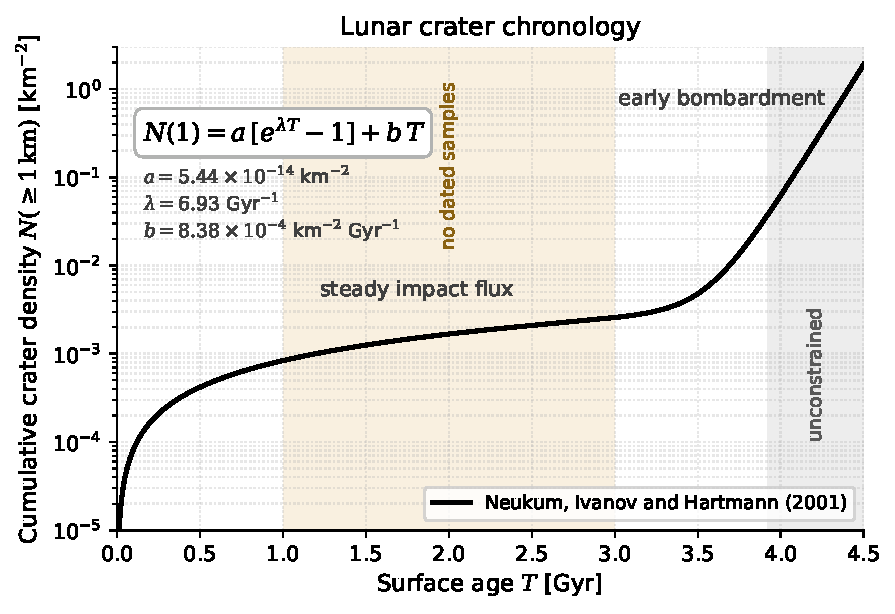
\includegraphics[width=0.62\linewidth]{figures/neukum_chronology_noreadoff}
\end{center}

\parti A lunar mare unit has a measured crater density $N(\geq 1\ \mathrm{km}) = 2.5 \times 10^{-3}\ \mathrm{km^{-2}}$.
On the young branch the linear term dominates, so compute the age from $N \approx b\,T$.
Then evaluate the exponential term at this age and show that it contributes only about $2\%$ of the measured density,
which justifies the approximation.

\begin{solution}
The linear inversion gives
\[
T = \frac{N}{b} = \frac{2.5 \times 10^{-3}}{8.38 \times 10^{-4}} = 2.9833\ \mathrm{Gyr}.
\]
At this age the exponential term is
\[
a\left[e^{\lambda T} - 1\right] = 5.44 \times 10^{-14} \times \left(e^{6.93 \times 2.9833} - 1\right)
= 5.44 \times 10^{-14} \times 9.5218 \times 10^{8} = 5.1799 \times 10^{-5}\ \mathrm{km^{-2}},
\]
which is $(5.1799 \times 10^{-5})/(2.5 \times 10^{-3}) \approx 2.1\%$ of the measured density.
Neglecting it overestimates the age by a comparable fraction, well below the systematic uncertainty of the method.
Note where this age lands on the figure: inside the shaded $1$--$3$ Gyr interval where no returned sample calibrates the curve,
so the result inherits the uncertainty of an interpolation.
\answer{$T = 2.9833\ \mathrm{Gyr}$, with the exponential term contributing $5.1799 \times 10^{-5}\ \mathrm{km^{-2}}$ ($\approx 2.1\%$ of the measured density). The linear approximation is well justified because this correction is far below the systematic uncertainty.}
\end{solution}

\parti A heavily cratered highlands unit has $N(\geq 1\ \mathrm{km}) = 3 \times 10^{-2}\ \mathrm{km^{-2}}$.
Read its approximate age off the figure.
Then refine it in two steps: neglect the linear term to obtain a first estimate
$T_0 = \lambda^{-1}\ln\!\left(1 + N/a\right)$,
then subtract the linear contribution $b\,T_0$ from $N$ and repeat.
Why does a factor-of-2 error in the measured $N$ barely change this age,
when the same error would double or halve the age in part (a)?

\begin{solution}
The figure gives $T \approx 3.9$ Gyr for $N = 3 \times 10^{-2}\ \mathrm{km^{-2}}$.
Neglecting the linear term:
\[
T_0 = \frac{1}{6.93}\ln\!\left(1 + \frac{3 \times 10^{-2}}{5.44 \times 10^{-14}}\right)
= \frac{\ln\!\left(5.5147 \times 10^{11}\right)}{6.93} = \frac{27.036}{6.93} = 3.9013\ \mathrm{Gyr}.
\]
The linear term at this age is $b\,T_0 = 8.38 \times 10^{-4} \times 3.9013 = 3.2693 \times 10^{-3}\ \mathrm{km^{-2}}$,
about $11\%$ of $N$. Subtracting it and inverting again:
\[
T_1 = \frac{1}{6.93}\ln\!\left(1 + \frac{2.6731 \times 10^{-2}}{5.44 \times 10^{-14}}\right) = 3.8846\ \mathrm{Gyr} \approx 3.885\ \mathrm{Gyr}.
\]
A further iteration changes the answer by less than $0.001$ Gyr, so the fixed point is reached.
The age is insensitive to $N$ because on the steep branch $N$ grows exponentially with $T$:
inverting, $T \sim \lambda^{-1}\ln(N/a)$, so a factor of 2 in $N$ shifts $T$ by only $\ln 2 / \lambda \approx 0.1$ Gyr
(explicitly, $N/2$ gives $3.77$ Gyr and $2N$ gives $3.99$ Gyr, a $\pm 3\%$ change).
In part (a) the relation is linear, $T = N/b$, so a factor of 2 in $N$ is a factor of 2 in age.
\answer{$T_0 = 3.9013\ \mathrm{Gyr}$ and refined age $T_1 = 3.8846\ \mathrm{Gyr} \approx 3.885\ \mathrm{Gyr}$. On the exponential branch $T \sim \lambda^{-1}\ln(N/a)$, so a factor of 2 in $N$ shifts $T$ by only $\approx 0.1$ Gyr ($\pm 3\%$).}
\end{solution}

\parti A fellow student writes: ``Plains unit A has twice the crater density of plains unit B, so A is twice as old.''
Judge this claim: in which regime is it correct, and in which two regimes does it fail?

\begin{solution}
The claim holds only on the linear branch of the chronology, for ages younger than about $3$ Gyr,
where the impact flux has been steady and $N \propto T$.
It fails in two regimes.
First, on the steep branch of the early bombardment, density is exponential in age:
as part (b) showed, a factor of 2 in $N$ there corresponds to an age difference of only about $0.1$ Gyr, not a factor of 2.
Second, at saturation: once craters overlap so densely that each new crater erases old ones,
$N$ stops growing entirely, and the lunar highlands are in this state.
Two saturated surfaces can differ greatly in age while showing the same crater density,
so beyond saturation crater counting sets only a lower limit on age.
\answer{The claim holds only on the linear branch younger than about $3$ Gyr ($N \propto T$). It fails on the steep exponential branch where a factor of 2 in $N$ is only about $0.1$ Gyr, and at saturation where crater counting sets only a lower limit on age.}
\end{solution}


% ════════════════════════════════════════════════════════════
\problem{Moment of inertia and the inside of Mercury}

The moment of inertia factor $C/MR^2$ is the single most informative number about a planet's interior:
it measures how strongly mass is concentrated toward the centre,
and it is measured from spin precession and gravity without ever drilling a hole.

\parti Model Mercury as a core of uniform density $\rho_c$ inside a mantle of uniform density $\rho_m$,
with core radius fraction $x = r_c/R = 0.83$ and core mass fraction $0.74$.
From the mean density, compute the two layer densities.

\begin{solution}
The core holds $74\%$ of the mass in a fraction $x^3$ of the volume, with $x^3 = 0.83^3 = 0.57179$:
\[
\rho_c = \frac{0.74\,\bar\rho}{x^3} = \frac{0.74 \times 5427}{0.57179} = \frac{4016.0}{0.57179} = 7023.6\ \mathrm{kg\,m^{-3}} \approx 7024\ \mathrm{kg\,m^{-3}}.
\]
The mantle holds the remaining $26\%$ of the mass in the remaining volume fraction $1 - x^3 = 0.42821$:
\[
\rho_m = \frac{0.26 \times 5427}{0.42821} = \frac{1411.0}{0.42821} = 3295.1\ \mathrm{kg\,m^{-3}} \approx 3295\ \mathrm{kg\,m^{-3}}.
\]
The core density is consistent with iron alloyed with lighter elements, and the mantle density with silicate rock:
the two-layer model recovers a physically sensible composition from three measured numbers.
\answer{$\rho_c = 7023.6\ \mathrm{kg\,m^{-3}} \approx 7024\ \mathrm{kg\,m^{-3}}$ and $\rho_m = 3295.1\ \mathrm{kg\,m^{-3}} \approx 3295\ \mathrm{kg\,m^{-3}}$. The core density is consistent with iron alloyed with lighter elements and the mantle with silicate rock.}
\end{solution}

\parti The two-layer moment of inertia factor is
\[
\frac{C}{MR^2} = \frac{2}{5}\,\frac{(f-1)\,x^5 + 1}{(f-1)\,x^3 + 1},
\qquad f = \frac{\rho_c}{\rho_m}.
\]
Evaluate it for your Mercury model,
compare with the measured value $0.346$,
and state in which direction the two-layer model errs and why.

\begin{solution}
The density contrast is $f = 7023.6/3295.1 = 2.1315$, and $x^5 = 0.83^5 = 0.39390$. Then
\[
\frac{C}{MR^2} = \frac{2}{5} \times \frac{1.1315 \times 0.39390 + 1}{1.1315 \times 0.57179 + 1}
= 0.4 \times \frac{1.4457}{1.6470} = 0.35111 \approx 0.3511.
\]
The model is about $1.5\%$ above the measured $0.346$: it errs toward the uniform-sphere value.
The reason is that each real layer compresses under its own weight,
so density rises toward the centre even within a chemically uniform layer,
and the true planet is more centrally condensed than any sharp two-layer model with constant layer densities.
The Lecture 8 notes' Earth example errs in the same direction ($0.345$ modelled against $0.331$ measured) and for the same reason.
\answer{$C/MR^2 = 0.35111 \approx 0.3511$, about $1.5\%$ above the measured $0.346$. The model errs toward the uniform-sphere value because real layers undergo self-compression, concentrating mass more strongly toward the centre.}
\end{solution}

\parti A fellow student writes: ``The Moon's $C/MR^2 = 0.393$ is within $2\%$ of the uniform-sphere value $0.400$,
so the Moon cannot have differentiated into a core and a mantle.''
Judge this claim, supporting your argument with the two-layer formula and the lunar core radius from the data block.

\begin{solution}
The claim is wrong, because a small core barely moves the moment of inertia factor.
Take the upper end of the lunar core radius range, $r_c = 380$ km, so $x = 380/1737 = 0.219$:
the core then fills only $x^3 \approx 0.0105$, about $1\%$ of the Moon's volume.
Even for a density contrast as large as $f = 2$, the two-layer formula gives
\[
\frac{C}{MR^2} = 0.4 \times \frac{1 + x^5}{1 + x^3} = 0.4 \times \frac{1.0005}{1.0105} = 0.396,
\]
already close to the measured $0.393$.
So a differentiated Moon with a small dense core predicts almost exactly the observed value:
$0.393$ is measurably below $0.400$ (the GRAIL and lunar laser ranging determination is far more precise than this difference),
and the deficit is the signature of a small core, not the absence of one.
The correct conclusion is the one in the Lecture 8 notes: the Moon is weakly differentiated,
with a core of only $200$--$380$ km, consistent with its origin from the silicate-rich debris of a giant impact.
\answer{False: a core of $200$ to $380$ km filling only about $1\%$ of the volume gives $C/MR^2 = 0.396$, close to the measured $0.393$. The deficit below $0.400$ is the signature of a small core, not the absence of one.}
\end{solution}


% ════════════════════════════════════════════════════════════
\problem{Central pressure}

Hydrostatic equilibrium plus a density profile determines the pressure everywhere inside a planet.
The uniform-density estimate is the standard first approximation, and its failure is itself instructive.

\parti Starting from hydrostatic equilibrium,
\[
\frac{\dd P}{\dd r} = -\frac{G\,m(r)\,\rho}{r^2},
\]
assume a uniform density $\rho$ and show that
\[
P(r) = \frac{2\pi}{3}\,G \rho^2 \left(R^2 - r^2\right),
\qquad
P_c = \frac{2\pi}{3}\,G \rho^2 R^2 = \frac{3\,G M^2}{8\pi R^4}.
\]

\begin{solution}
For uniform density the enclosed mass is $m(r) = \frac{4}{3}\pi \rho r^3$, so
\[
\frac{\dd P}{\dd r} = -\frac{G \rho}{r^2}\,\frac{4}{3}\pi \rho r^3 = -\frac{4\pi}{3}\,G \rho^2 r.
\]
Integrating from $r$ to the surface, where $P(R) = 0$:
\[
P(r) = \frac{4\pi}{3}\,G\rho^2 \int_r^R r'\,\dd r' = \frac{2\pi}{3}\,G \rho^2 \left(R^2 - r^2\right).
\]
At the centre, $P_c = \frac{2\pi}{3} G \rho^2 R^2$. Substituting $\rho = 3M/(4\pi R^3)$:
\[
P_c = \frac{2\pi}{3}\,G\,\frac{9 M^2}{16 \pi^2 R^6}\,R^2 = \frac{3\,G M^2}{8\pi R^4},
\]
as required. The central pressure of a uniform body depends only on its mass and radius.
\answer{$P(r) = \frac{2\pi}{3}\,G \rho^2 (R^2 - r^2)$ and $P_c = \frac{3\,G M^2}{8\pi R^4}$. The central pressure of a uniform body depends only on its mass and radius.}
\end{solution}

\parti Evaluate the mean density of Mars,
then its central pressure.

\begin{solution}
With $M = 6.417 \times 10^{23}$ kg and $R = 3.3895 \times 10^{6}$ m:
\[
\bar\rho = \frac{3M}{4\pi R^3} = \frac{6.417 \times 10^{23}}{1.63116 \times 10^{20}} = 3934.0\ \mathrm{kg\,m^{-3}},
\]
matching the value in the Lecture 8 notes. The central pressure follows from $M^2 = 4.1178 \times 10^{47}\ \mathrm{kg^2}$ and $R^4 = 1.3199 \times 10^{26}\ \mathrm{m^4}$:
\[
P_c = \frac{3\,G M^2}{8\pi R^4} = \frac{2.0022 \times 10^{-10} \times 4.1178 \times 10^{47}}{25.133 \times 1.3199 \times 10^{26}}
= 2.4853 \times 10^{10}\ \mathrm{Pa} \approx 24.9\ \mathrm{GPa}.
\]
As a cross-check, $\frac{2\pi}{3} G \bar\rho^2 R^2$ gives the same number.
Mars's central pressure is about seven times smaller than the same estimate for Earth ($\approx 170$ GPa):
the strong scaling $P_c \propto M^2/R^4$ separates even neighbouring planets by large factors.
\answer{$\bar\rho = 3934.0\ \mathrm{kg\,m^{-3}}$ and $P_c = 2.4853 \times 10^{10}\ \mathrm{Pa} \approx 24.9\ \mathrm{GPa}$. Mars's central pressure is about seven times smaller than Earth's ($\approx 170$ GPa) because of the strong $P_c \propto M^2/R^4$ scaling.}
\end{solution}

\parti For Earth the same estimate gives $P_c \approx 170$ GPa, while the true central pressure is about $360$ GPa.
Explain why the uniform-density formula systematically underestimates the central pressure of a differentiated planet,
and state whether your Mars value from part (b) is a lower or an upper bound on the true martian central pressure.

\begin{solution}
The uniform model spreads the planet's mass evenly, but a differentiated planet concentrates
its densest material (the iron core) at depth.
The pressure gradient scales with the local density and the enclosed mass;
concentrating mass toward the centre raises both factors exactly where the pressure is built up,
so the integrated central pressure exceeds the uniform estimate.
For Earth the effect is roughly a factor of 2 ($170$ against $\approx 360$ GPa).
Mars is also differentiated, with a liquid iron-alloy core, so the part (b) value is a lower bound:
the true martian central pressure is larger than $25$ GPa.
The size of the correction grows with the degree of central condensation,
so it is largest for Earth ($C/MR^2 = 0.331$) and smallest for nearly uniform bodies like the Moon ($0.393$).
\answer{The uniform formula is a lower bound, so the true martian central pressure is larger than $25$ GPa. Central condensation concentrates mass and raises local density at depth, increasing the true central pressure above the uniform estimate (a factor of 2 for Earth, $170$ against $\approx 360$ GPa).}
\end{solution}


% ════════════════════════════════════════════════════════════
\problem{Seismology: listening to interiors}

Seismic waves are the sharpest probe of planetary interiors:
what arrives, what is missing, and where it is missing all encode the deep structure.
No numbers are needed in this problem; the reasoning is the exam skill.

\parti On Earth, direct S waves are absent everywhere beyond about $103^\circ$ from an earthquake,
while P waves are missing only in a ring between about $103^\circ$ and $143^\circ$.
Explain the different physical cause of each shadow zone,
and state what the S-wave shadow proves about the outer core.

\begin{solution}
S waves are shear waves: they require a nonzero shear modulus, and a liquid has none.
Any ray path that touches the outer core is therefore absorbed,
so no direct S wave reaches any station beyond the tangent ray at about $103^\circ$: the S shadow is total.
P waves are compressional and do propagate through liquid,
but the compressional wave speed drops sharply at the core-mantle boundary
(from about $13.7$ to about $8.1\ \mathrm{km\,s^{-1}}$),
so rays entering the core refract steeply downward.
This bending deflects arrivals away from the band between about $103^\circ$ and $143^\circ$,
a shadow of refraction rather than absorption, and beyond $143^\circ$ core-traversing P waves reappear.
The totality of the S shadow is the definitive evidence that the outer core is liquid.
\answer{The total S shadow beyond about $103^\circ$ is due to shear absorption, proving the outer core is liquid. The P shadow between about $103^\circ$ and $143^\circ$ is due to downward refraction as wave speed drops from about $13.7$ to about $8.1\ \mathrm{km\,s^{-1}}$.}
\end{solution}

\parti InSight's marsquake data show that at the martian core-mantle boundary
the S-wave speed drops to zero while the P-wave speed steps down rather than up.
State what each feature implies for the state and the composition of the martian core.

\begin{solution}
The vanishing of $v_S$ at the boundary means the shear modulus vanishes: the martian core is liquid,
exactly as Earth's S-wave shadow zone demonstrates for the outer core.
The compositional information is in the downward step of $v_P$.
The compressional speed is set by the bulk modulus and the density,
and a liquid iron-sulfur alloy has a smaller bulk modulus than the overlying solid silicate mantle,
so $v_P$ decreases across the boundary even though the density increases.
Together the two profiles identify a liquid core of iron alloyed with a substantial fraction
of light elements, particularly sulfur, less dense than Earth's outer core.
\answer{Vanishing $v_S$ proves the martian core is liquid, while the downward step in $v_P$ indicates a lower bulk modulus than the silicate mantle. Together they identify a liquid core of iron alloyed with light elements, particularly sulfur.}
\end{solution}

\parti A fellow student writes: ``PREM shows the density jumping from about $5570$ to about $9900\ \mathrm{kg\,m^{-3}}$
at the core-mantle boundary, but the Adams-Williamson equation predicts a smooth profile there;
the equation must be wrong.''
Judge this claim.

\begin{solution}
The claim misreads what the equation asserts.
The Adams-Williamson relation propagates density downward under two explicit assumptions:
uniform composition and adiabatic self-compression.
Where those assumptions hold, it works: through the lower mantle it reproduces the PREM density profile closely,
because there the density rise is dominated by self-compression.
At the core-mantle boundary the composition changes from silicate rock to iron alloy,
so the uniform-composition assumption fails by construction, and the equation is not expected to apply across the jump.
Far from refuting the equation, the deviation is the measurement:
the mismatch between the smooth Adams-Williamson extrapolation and the observed jump
is precisely how the compositional layering of the deep interior is exposed.
An equation used outside its stated assumptions is not wrong; it is a diagnostic.
\answer{The claim is false: Adams-Williamson assumes uniform composition, which holds within the mantle but fails across the core-mantle boundary where density jumps from about $5570$ to about $9900\ \mathrm{kg\,m^{-3}}$. The mismatch is a diagnostic that exposes compositional layering.}
\end{solution}
